
\section{Summary of Data Sets}\label{sec:data-summary}

In \Cref{tab:dataset-info} we summarize the data sets we use in our paper.

\begin{table}
  \centering
  \caption{Details of the real datasets used in the experiments, The median \(q\) value
    refers to the median of the proportion of ones for the binary features in the data. Note that in the case of \data{housing}, there is
    only a single binary feature.}
  \label{tab:dataset-info}
  \vskip 0.15in
  \begin{tabular}{
      l
      S[table-format=4.0]
      S[table-format=4.0]
      l
      l
      S[table-format=1.3,round-mode=places,round-precision=3]
    }
    \toprule
    Dataset   & {\(n\)} & {\(p\)} & Response   & Design     & {Median \(q\)} \\
    \midrule
    a1a       & 1605    & 123     & binary     & binary     & 0.970093       \\
    w1a       & 2477    & 300     & binary     & binary     & 0.976181       \\
    rhee2006  & 842     & 361     & continuous & binary     & 0.995249       \\
    housing   & 506     & 13      & continuous & mixed      & 0.93083        \\
    leukemia  & 38      & 7129    & binary     & continuous &                \\
    triazines & 186     & 60      & continuous & mixed      & 0.973118       \\
    \bottomrule
  \end{tabular}
\end{table}

We also summarize the distribution of class balance among all the binary features in
\Cref{fig:data-hist-q}. Note that the clas imbalance for these data sets is quite severe.
We want to emphasize that this is not the result of cherry-picking. It is common for data
sets, particularly high-dimensional ones, to have many imbalanced features. We did not look
at the class balances when picking these data sets, neither have any other data sets ever
been considered for our experiments.

\begin{figure}[htpb]
  \centering
  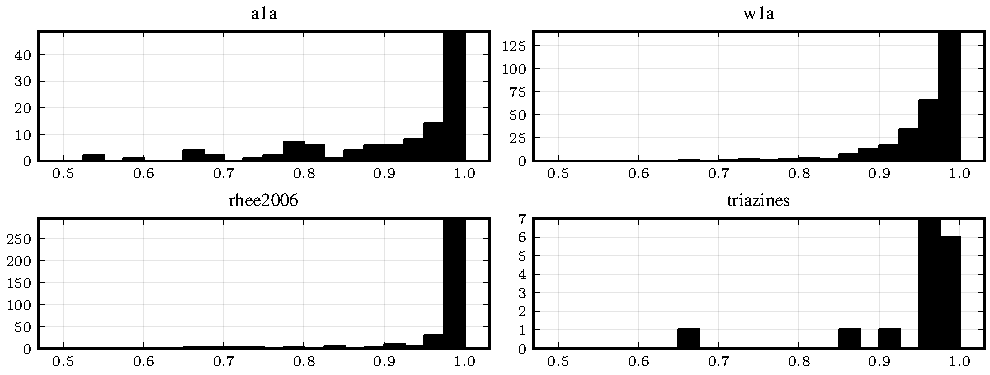
\includegraphics[]{plots/data-hist-q.pdf}
  \caption{%
    Histograms over the distribution of \(q\) (class balance, that is, the
    proportion of ones) for the binary features in each of the data sets
    used in the paper.
  }
  \label{fig:data-hist-q}
\end{figure}

